\documentclass[../bryant_comp_sys.tex]{subfiles}
\begin{document}
    \chapter{Representing and Manipulating Information}
        \begin{outline}
            \1 Computer process information as binary signals called \glspl{bit}
            \1 Individual bits are meaningless, sets of bits have meaning.
            \1 Three important representations of numbers:
                \2 \textbf{Unsigned}: Based on traditional binary notation, represent numbers greater than or equal to 0.
                \2 \textbf{Two's--complement}: Represent signed real numbers.
                \2 \textbf{Floating--point}: Base--two representation of scientific notation, for real numbers.
            \1 Limited numbers of bits are used to represent numbers. Going over this can cause an \gls{overflow}
            \1 \alert{important}: Floating--point arithmetic is not associative, as precision is not infinite.
                \2 Example: \((3.14 + 1\text{E}20) - 1\text{E}20\) will most likely evaluate to \(0.0\) on most machines, whereas \(3.14 + (1\text{E}20 - 1\text{E}20)\) usually evaluates to 3.14.
                \2 Integers encode a narrow range of numbers precisely, floating--point numbers encode a wide range approximately.
        \end{outline}

        \section{Information Storage}
            \begin{outline}
                \1 Information is stored in eight bit blocks called a \gls{byte}. A program views memory as a large array of bytes, called its \gls{vram}
                \1 Every byte is identified by a unique number called an \gls{address}, the set of which compose virtual address space.
                \1 All allocation and management of memory at the program level is done in virtual address space.
                    \2 Languages associate type information (e.g. \texttt{int}) with each byte of memory it uses, but the machine--level program the languages generate have no type information themselves.
            \end{outline}

            \subsection{Hexadecimal Notation}
                \begin{outline}
                    \1 A value of a byte ranges from \(00000000_2\) to \(11111111_2\) in binary notation and from \(0_{10}\) to \(255_{10}\) in decimal integer notation.
                    \1 Writing numbers in binary notation is tedious, use base--16 numbers, called \gls{hex}
                        \2 A value of a single byte ranges from \(00_{16}\) to \(FF_{16}\)
                        \2 A hex number is denoted by a starting string, either \texttt{0x} or \texttt{0X}
                    \1 A lot of stuff about interconverting between them, but I won't replicate it here (pp. 34-37)
                \end{outline}

            \subsection{Words}
                \begin{outline}
                    \1 Computers have different word sizes, which indicate the nominal size of integer and pointer data.
                    \1 Puts a maximum limit on virtual address space: a machine with a word size of \(w\) has virtual addresses on the interval \(\left[ 0, 2^w - 1 \right]\), giving a program access to \(2^w\) bytes
                        \2 This is why 32--bit machines are capped at 4 GB of RAM (\(2^{32} \simeq 4.3 \times 10^{9}\) bytes)
                \end{outline}

            \subsection{Data Sizes}
                \begin{outline}
                    \1 Machines have instructions for manipulating blocks of memory on 1, 2, 4, and 8 byte intervals.
                    \1 Language types have different byte sizes (see \fref{tab:typeSizes} for C/\Cpp type sizes)
                    \begin{table}[]
                        \centering
                        \begin{tabular}{lcc}
                          C/\Cpp type               & 32--bit   & 64--bit   \\ \hline
                          \texttt{char}             & 1         & 1         \\
                          \texttt{short int}        & 2         & 2         \\
                          \texttt{int}              & 4         & 4         \\
                          \texttt{long int}         & 4         & 8         \\
                          \texttt{long long int}    & 8         & 8         \\
                          \texttt{char*}            & 4         & 8         \\
                          \texttt{float}            & 4         & 4         \\
                          \texttt{double}           & 8         & 8
                        \end{tabular}
                        \label{tab:typeSizes}
                        \caption{Type sizes in bytes for various C/\Cpp types}
                        \end{table}
                \end{outline}

            \subsection{Addressing and Byte Ordering}
                \begin{outline}
                    \1 Two conventions must be established to make things consistent:
                        \2 What the address of an object will be
                        \2 How bytes are ordered in memory
                    \1 A multi--byte object is stored as a contiguous sequence of bytes
                        \2 The object's address is the smallest address of the bytes it spans
                    \1 Assume we have a \(w\)--bit object with the bit representation \(\left[ x_{w-1}, x_{w-2}, \ldots, x_1, x_0 \right]\), where \(x_{w-1}\) is the most significant bit and \(x_0\) is the least.
                        \2 If \(w\) is a byte (multiple of 8), the bits can be grouped as bytes, with \(\left[ x_{w-1}, x_{w-2}, \ldots, x_{w-8} \right]\) being the most significant byte and  \(\left[ x_{7}, x_{6}, \ldots, x_{w-0} \right]\) being the least
                        \2 Two conventions fr ordering bytes (\Fref{fig:endian}):
                            \3 \textbf{\Gls{littleend}}: The least significant byte is listed first
                            \3 \textbf{\Gls{bigend}}: The most significant byte is listed first
                            
                    \begin{figure}
                        \centering
                        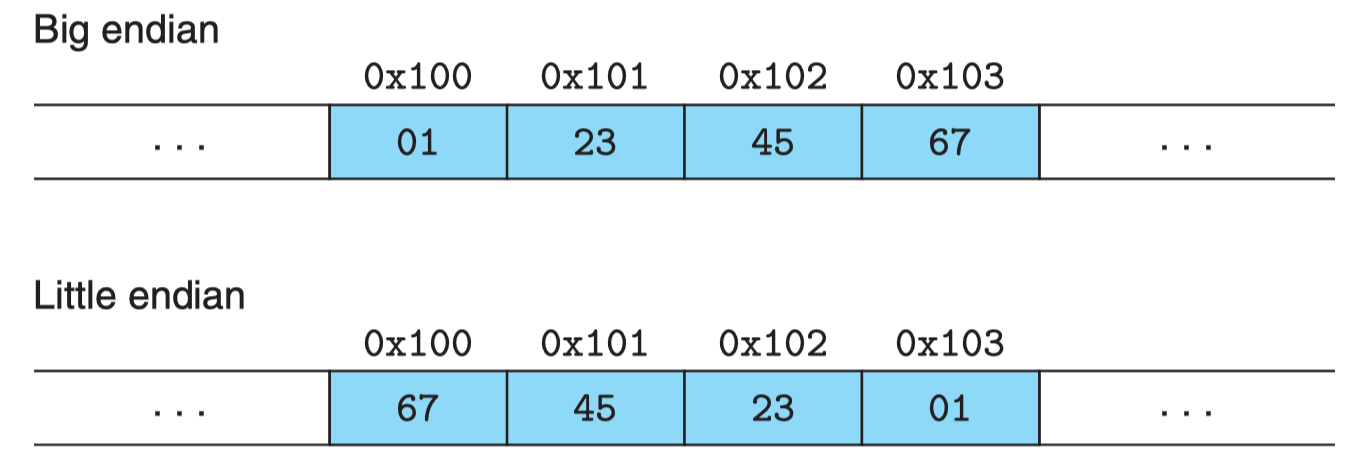
\includegraphics[width=0.5\linewidth]{ch2/figs/endian.png}
                        \label{fig:endian}
                        \caption{Different conventions for bit ordering.}
                    \end{figure}

                        \2 Most modern processors are \textit{bi-endian}
                        \2 Bit ordering is usually unimportant, but there are several cases where it is critical to know which one is being used:
                            \3 Binary data transfer between two machines over a network
                            \3 When looking at machine--level code (such as decompiled C/\Cpp code)
                            \3 When circumventing a language's typing, e.g. using \texttt{cast} in C/\Cpp
                \end{outline}
            
            \subsection{Representing Strings}
                \begin{outline}
                    \1 In C, a string is represented as an array of characters terminated by a null character, \texttt{\\0}
                    \1 Text is more platform independent than binary data
                \end{outline}
            
            \subsubsection{Representing Code}
                \begin{outline}
                    \1 Different machine types have different and incompatible instruction codings
                        \2 For the function below, \Fref{tab:encodings} show the different machine--level encodings for some architectures

                        \lstset{language=C++}
                        \begin{lstlisting}
                            int sum(int x, int y)
                            {
                                return x + y;
                            }
                        \end{lstlisting}
                            
                    \begin{table}[h!]
                        \centering
                        \begin{tabular}{ll}
                            \textbf{Linux 32}   & \texttt{55 89 e5 8b 45 0c 03 45 08 c9 c3}              \\
                            \textbf{Linux 64}   & \texttt{55 48 89 e5 89 7d fc 89 75 f8 03 45 fc c9 c3}  \\
                            \textbf{Sun}        & \texttt{81 c3 e0 08 90 02 00 09}                       \\
                            \textbf{Windows}    & \texttt{55 89 e5 8b 45 0c 03 45 08 5d c3}
                        \end{tabular}
                        \label{tab:encodings}
                        \caption{Different machines have different character encodings.}
                    \end{table}

                    \1 \alert{important}: The computer has no information about the original program it's running, everything is just bits to it.
                \end{outline}

            \subsubsection{Introduction to Boolean Algebra}
                \begin{outline}
                    \1 Most of this is just review for me, so I won't discuss a lot of it 

                    \begin{table}[h!]
                        \centering
                        \begin{tabular} {ccc}
                            Operation           & Math Symbol   & Meaning               \\ \hline
                            \(\sim\)            & \(\neg\)      & not                   \\
                            \&                  & \(\land\)     & and                   \\
                            \(\mid\)            & \(\lor\)      & or                    \\
                            \textasciicircum    & \(\oplus\)    & exclusive--or (xor)
                        \end{tabular}
                        \label{tab:boolsymbols}
                        \caption{Boolean symbols and their meaning}
                    \end{table}

                    \1 The boolean operations can also operate on \textit{bit vectors}, strings of binary numbers of a fixed length \(w\)
                        \2 Example: let \(a\) and \(b\) be the bit vectors \(\left[ a_{w-1}, a_{w-2}, \ldots, a_0 \right]\) and \(\left[ b_{w-1}, b_{w-2}, \ldots, b_0 \right]\)
                        \2 \(a \& b\) is a bit vector of length \(w\) where the \(i\)th element is \(a_i \& b_i\)
                    \1 Goes on to describe some bitwise and logical operations, which I will not replicate.
                \end{outline}

        \section{Integer Representations}
            \begin{outline}
                \1 Describes two different ways bits can be used to encode integers, unsigned and signed.
            \end{outline}

            \subsection{Integral Data Types}
                \begin{outline}
                    \1 \textit{Integral data types}: types which represent finite ranges of integers. \Fref{tab:integralData} shows the guaranteed range of integral data types (guaranteed on both 32-- and 64--bit systems)
                        \2 The guaranteed ranges differ from the ``typical ranges'' (shown on pg. 57), in that several data types have different maximums (notably \texttt{unsigned long int}), and the symmetric range of the negative and positive extrema
                    \begin{table}[]
                        \centering
                        \begin{tabular}{lrr}
                            C/\Cpp~Data Type & Minimum & Maximum \\ \hline
                            \texttt{char}                   & -127                          & 127 \\
                            \texttt{unsigned char}          & 0                             & 255 \\
                            \texttt{short int}              & -32 767                       & 32 767 \\
                            \texttt{unsigned short int}     & 0                             & 65 535 \\
                            \texttt{int}                    & -32 767                       & 32 767 \\
                            \texttt{unsigned int}           & 0                             & 65 636 \\
                            \texttt{long int}               & -2 147 483 647                & 2 147 483 647 \\
                            \texttt{unsigned long int}      & 0                             & 4 294 967 295 \\
                            \texttt{long long int}          & -9 223 372 036 854 775 807    & 9 223 372 036 854 775 807 \\
                            \texttt{unsigned long long int} & 0                             & 18 446 744 073 709 551 615
                        \end{tabular}
                        \label{tab:integralData}
                        \caption{Guaranteed ranges of C/\Cpp~integral types.}
                    \end{table}
                \end{outline}

            \subsubsection{Unsigned Encodings}
                \begin{outline}
                    \1 Assume we have an integer data type of \( w \) bits and a bit vector, \( \overrightarrow{x} \), \( \left[ x_{w-1}, x_{w-1}, \ldots, x_0 \right] \)
                        \2 If we treat \( \overrightarrow{x} \) as a number written in binary, this is the \gls{unsigned} interpretation of \( \overrightarrow{x} \), expressed as 
                        \[
                            B2U_{w}(\overrightarrow{x}) \doteq \sum_{i=0}^{w-1} x_i 2^i
                        \]
                        where \( B2U_w \) means ``binary to unsigned'' of length \( w \) and ``\( \doteq \)'' means ``defined as''.
                        \2 This can be thought of as a mapping of sets of ones and zeros to nonnegative integers.
                            \3 For example,
                            \begin{align*}
                                B2U_4(\left[ 0001 \right]) &= \left( 0 \times 2^3 \right) + \left( 0 \times 2^2 \right) + \left( 0 \times 2^1 \right) + \left( 1 \times 2^0 \right) = 0 + 0 + 0 + 1 = 1 \\
                                B2U_4(\left[ 0101 \right]) &= \left( 0 \times 2^3 \right) + \left( 1 \times 2^2 \right) + \left( 0 \times 2^1 \right) + \left( 1 \times 2^0 \right) = 0 + 4 + 0 + 1 = 5
                            \end{align*}
                    \1 The unsigned binary representation is important in that every number in its interval, \( \left[ 0, 2^{w-1} \right] \), has a unique encoding as a \( w \)--bit value.
                        \2 This means the function \( B2U_w \) is a \textit{bijection}; every bit vector of length \( w \) is associated with a unique value
                \end{outline}

            \subsubsection{Two's--Complement Encodings}
                \begin{outline}
                    \1 \Gls{twoCom} is the common computer representation of signed numbers
                        \2 Defined by interpreting the most significant bit of the word to have a negative weight,
                            \[
                                B2T_{w}(\overrightarrow{x}) \doteq -x_{w-1}2^{w-1} + \sum_{i=0}^{w-2} x_i 2^i
                            \]
                        \2 This negative weight bit is called the \textit{sign bit}. The encoded number is negative when the sign bit is set to 1, and positive when it is set to 0.
                        \2 Below show two example maps
                            \begin{align*}
                                B2U_4(\left[ 0101 \right]) &= \left( 0 \times 2^3 \right) + \left( 1 \times 2^2 \right) + \left( 0 \times 2^1 \right) + \left( 1 \times 2^0 \right) = 0 + 4 + 0 + 1 = 5 \\
                                B2U_4(\left[ 1011 \right]) &= \left( -1 \times 2^3 \right) + \left( 0 \times 2^2 \right) + \left( 1 \times 2^1 \right) + \left( 1 \times 2^0 \right) = -8 + 0 + 2 + 1 = -5
                            \end{align*}
                            \3 Note that the mapping for \( 5 \) and \( -5 \) are \textbf{not} symmetric.
                    \1 What is the range of values this method can encode?
                        \2 The smallest representable number is the bit vector \( \left[ 10 \cdots 0 \right] \), with an integer value of \( T_{\text{min}, w} \doteq -2^{w-1} \), and the largest representable number is the bit vector \( \left[ 01 \cdots 1\right] \), with an integer value of \( T_{\text{max}, w} \doteq \sum_{i=0}^{w-2} 2^1 = 2^{w-1} - 1 \)
                        \2 With a 4--bit vector, \( T_{\text{min}, w} = -8 \) and \( T_{\text{max}, w} = 7 \)
                        \2 \( \therefore~B2T_{w}: \{0,1\}^w \rightarrow \{-2^{w-1}, \ldots, 2^{w-1} - 1\} \)
                        \2 As with the unsigned encoding, \( B2T_w \) is a bijection (each bit vector has a unique encoding)
                \end{outline}

            \subsubsection{Conversions Between Signed and Unsigned Encodings}
                \begin{outline}
                    \1 \alert{important}: C/\Cpp handles casting on the bit--level: casting between signed and unsigned encodings keeps the bit values identical but changes how they are interpreted.
                        \2 Suppose we have the bit vector \( \left[ 1011 \right] \).
                            \3 In two's--complement, the first bit, the sign bit, is interpreted as \( -8 \), whereas in an unsigned encoding it is interpreted as \( +8 \). So the negative values in two's--complement are increased by \( 2^4 = 16 \) in an unsigned encoding (\(-5\) becomes \(+11\)).
                    \1 When mapping a signed number to its unsigned counterpart, negative numbers are converted to large positive numbers and positive numbers remain unchanged. When going from unsigned to signed, large numbers ( \( >2^{w-1} \), the maximum value for signed numbers) go to negative values and numbers \( <2^{w-1} \) remain unchanged (\Fref{fig:encodingConversions}).

                    \begin{figure}[h]
                        \centering
                        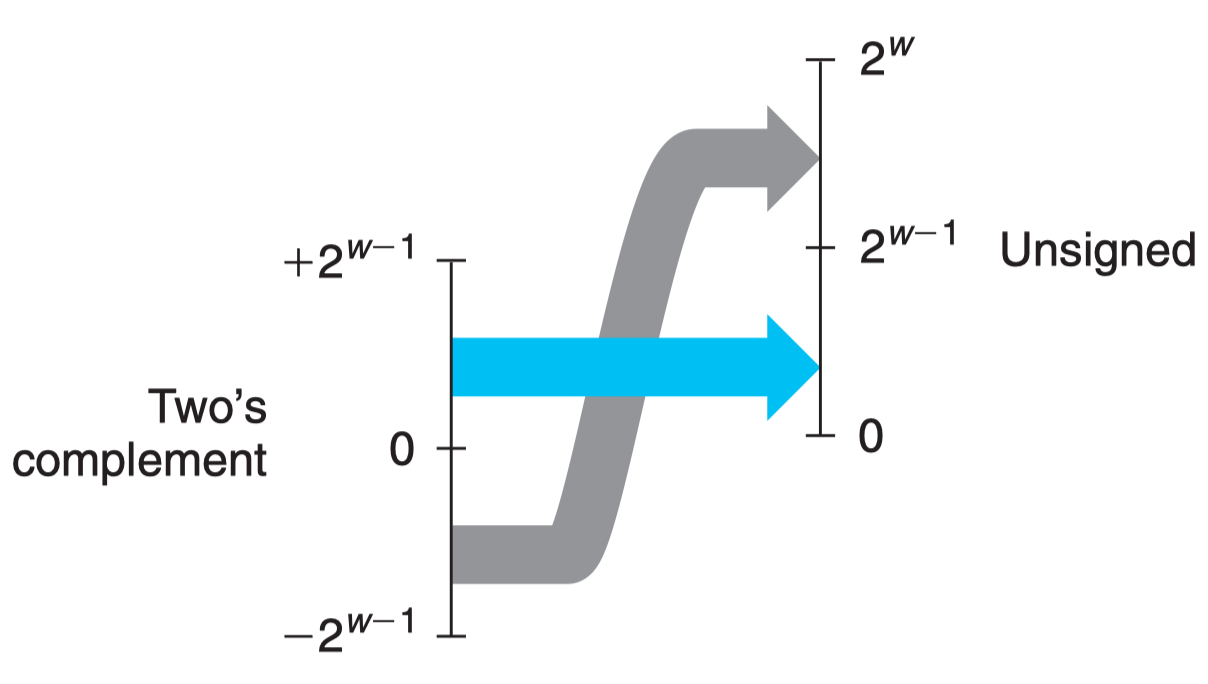
\includegraphics[width=0.4\linewidth]{ch2/figs/signed_to_unsigned.png}
                        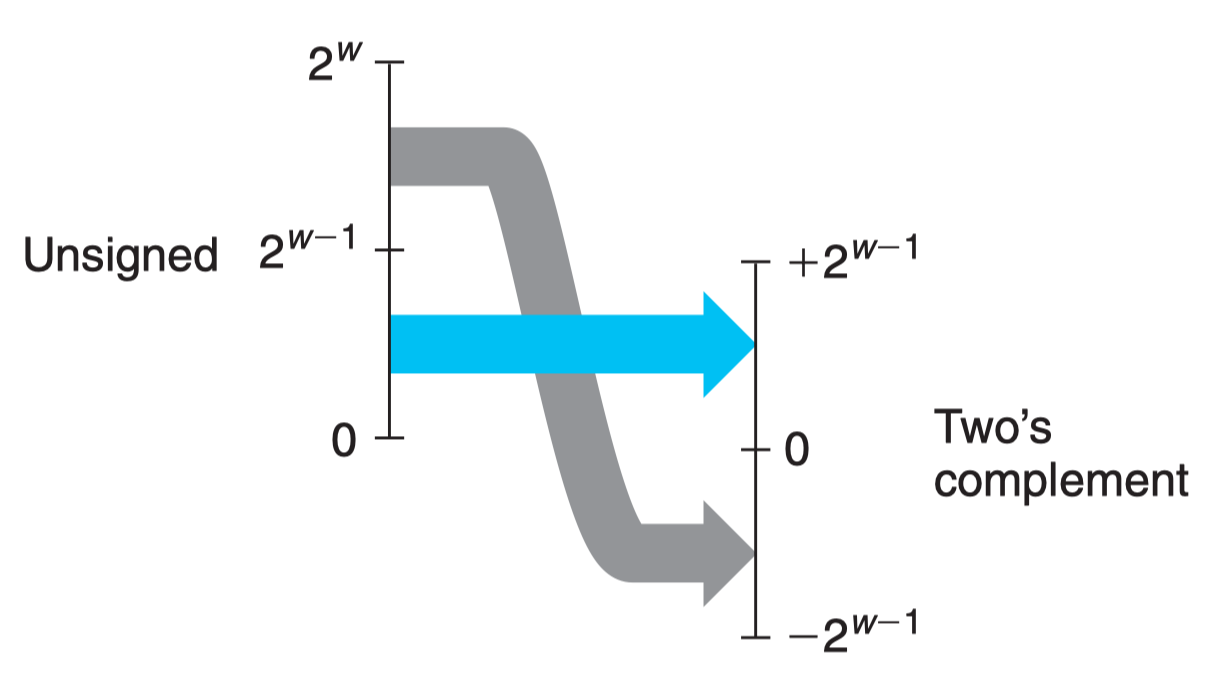
\includegraphics[width=0.4\linewidth]{ch2/figs/unsigned_to_signed.png}
                        \caption{Interconversions between signed and unsigned numbers.}
                        \label{fig:encodingConversion}
                    \end{figure}

                    \1 \alert{important}: When handling an operation when one number is signed and the other is unsigned, C/\Cpp~implicitly casts the signed argument to an unsigned, and performs the operation assuming both numbers are non--negative.
                \end{outline}

            \subsubsection{Expanding the Bit Representation of a Number}
                \begin{outline}
                    \1 This subsection deals with converting between integers with different word sizes while retaining their values.
                    \1 Converting an unsigned number to a larger data type, we add leading zeros to the bit--level representation, called \gls{zeroExt}.
                    \1 Converting a two's--complement number to a larger data type is performed by doing \gls{signExt}, or adding leading copies of the sign bit, 0 or 1.
                        \2 Assume our original value has the bit--level representation \( \left[ {\color{cyan} x_{w-1}}, x_{w-2}, \ldots, x_0 \right] \), the extended bit--level representation is then \( \left[ {\color{cyan} x_{w-1}}, \ldots, {\color{cyan} x_{w-1}}, {\color{cyan} x_{w-1}}, x_{w-2}, \ldots, x_0 \right] \)
                    \1 Goes on to show a proof that sign extension works properly (pp. 72---74)
                    \1 There's an order of operations, e.g. when going from a \texttt{short} to an \texttt{unsigned}, first change the size then change the sign, \texttt{short} \( \rightarrow \) \texttt{int} \( \rightarrow \) \texttt{unsigned}
                \end{outline}

            \subsubsection{Truncating Numbers}
                \begin{outline}
                    \1 When truncating a \textit{w}--bit number \( \hat{x} = \left[ x_{w-1}, x_{w-1}, \ldots, x_0 \right] \) to a \textit{k}--bit number, we drop the high order \( w - k \) bits to produce the bit--vector \( \hat{x}^{\prime} = \left[ x_{k-1}, x_{k-2}, \ldots, x_0 \right] \)
                    \1 Truncation can alter the value of a number, which is a form of overflow
                    \1 For an unsigned integer \( x \), the result of truncation to \( k \)--bits is equal to \( x~\text{mod}~2^k \)
                        \2 Signed integers can be treated similarly
                        \2 So, for unsigned truncation:
                        \[
                            B2U_k \left( \left[ x_{k-1}, x_{k-2}, \ldots, x_0 \right] \right) = B2U_w \left( \left[ x_{w-1}, x_{w-2}, \ldots, x_0 \right] \right)~\text{mod}~2^k
                        \]
                        and for signed truncation:
                        \[
                            B2T_k \left( \left[ x_{k-1}, x_{k-2}, \ldots, x_0 \right] \right) = U2T_k \left( B2U_w \left( \left[ x_{w-1}, x_{w-2}, \ldots, x_0 \right] \right)~\text{mod}~2^k \right)
                        \]
                \end{outline}

            \section{Integer Arithmetic}
                \begin{outline}
                    \1 A lot of the strangeness around mathematical operations in code, such as the possibility of the addition of two positive integers producing a negative number, can be traced back to the finite nature of computer arithmetic
                \end{outline}

                \subsection{Unsigned Addition}
                    \begin{outline}
                        \1 Assume we have two non--negative integers \( x \) and \( y \), such that \( 0 \leq x \) and \( y \leq 2^{w-1} \)
                            \2 If both of these numbers are represented as \( w \)--bit unsigned numbers, the addition of the two would be in the range \( 0 \leq x + y \leq 2^{w+1} - 2 \), requiring up to \( w+1 \) bits.
                            \2 If we add a number to this \( w+1 \)--bit number, we may require \( w+2 \) bits, and so on. this is called \textit{word--size inflation}
                        \1 \alert{important}: Unsigned arithmetic is equivalent to computing the sum modulo \( 2^w \)
                            \2 Computed by discarding the high--order bit in the \( w+1 \)--bit representation of \( x+y \)
                            \2 If \( x+y < 2^w \), the leading bit in the \( w+1 \)--bit representation is 0, so the value is unchanged upon discarding it
                            \2 If the leading bit is 1, i.e. \( 2^w \leq x+y \leq 2^{w+1} \), the leading bit is 1, so discarding it is equivalent to subtracting \( 2^w \) from the sum
                            \2 Thus the result is
                            \[
                                x + \binom{u}{w}y = \begin{cases} x+y & x + y < 2^w \\ x + y-2^w & 2^w \leq x + y \leq 2^{w+1} \end{cases} 
                            \]
                            \2 If the result cannot fit into the word size, the operation \glspl{overflow}
                        \1 Modular addition is an \gls{abelian}, literally just commutative, and is also associative.
                    \end{outline}

                \subsection{Two's--Complement Addition}
                    \begin{outline}
                        \1 Must decide both when the result is too large (positive) or too small (negative)
                        \1 For integers \( x \) and \( y \) on the range \( -2^{w-1} \leq x,y \leq 2^{w-1}-1 \), their sum is in the range \( -2^w \leq x + y \leq 2^w - 2 \), again potentially requiring \( w+1 \) bits to represent
                            \2 Again, we truncate to \( w \) bits to avoid overflow
                        \1 Most computers use the same instructions to perform signed and unsigned addition, as the bit--level representation of a \( w \)--bit two's--complement sum is the same as the unsigned sum
                            \2 Thus, the two's--complement addition for a word--size \( w \), denote as \( +\binom{t}{w} \) on \( x, y \) in the range \( -2^{w-1} \leq x,y \leq 2^{w-1} \) is
                                \[
                                    x + \binom{t}{y}y \equiv U2T_w(T2U_w(x) + \binom{u}{w} T2U_w(y))
                                \]
                        \1 Similar to unsigned addition, the results for two's--complement addition is
                            \[
                                x + \binom{t}{w} = \begin{cases} x + y - 2^w & 2^{w-1} \leq x + y,~\text{positive overflow} \\ x + y & -2^{w-1} \leq x + y < 2^{w-1},~\text{okay} \\ x + y + 2^w & x + y < -2^{w-1},~\text{negative overflow}\end{cases}
                            \]
                        \1 Graphically,
                            \begin{figure}[h]
                                \centering
                                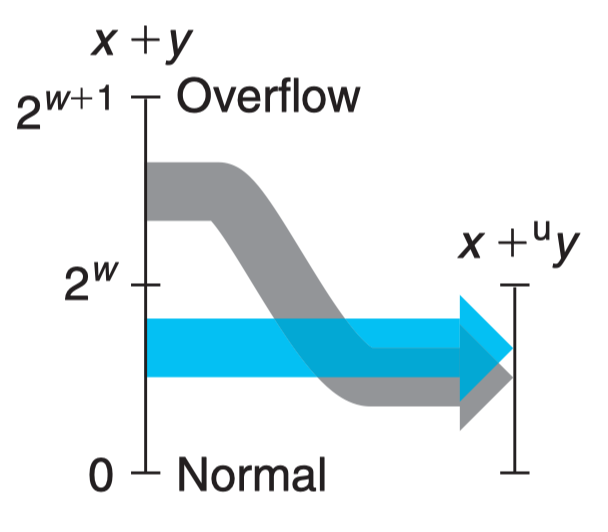
\includegraphics[width=0.25\linewidth]{ch2/figs/int_add_unsigned.png}
                                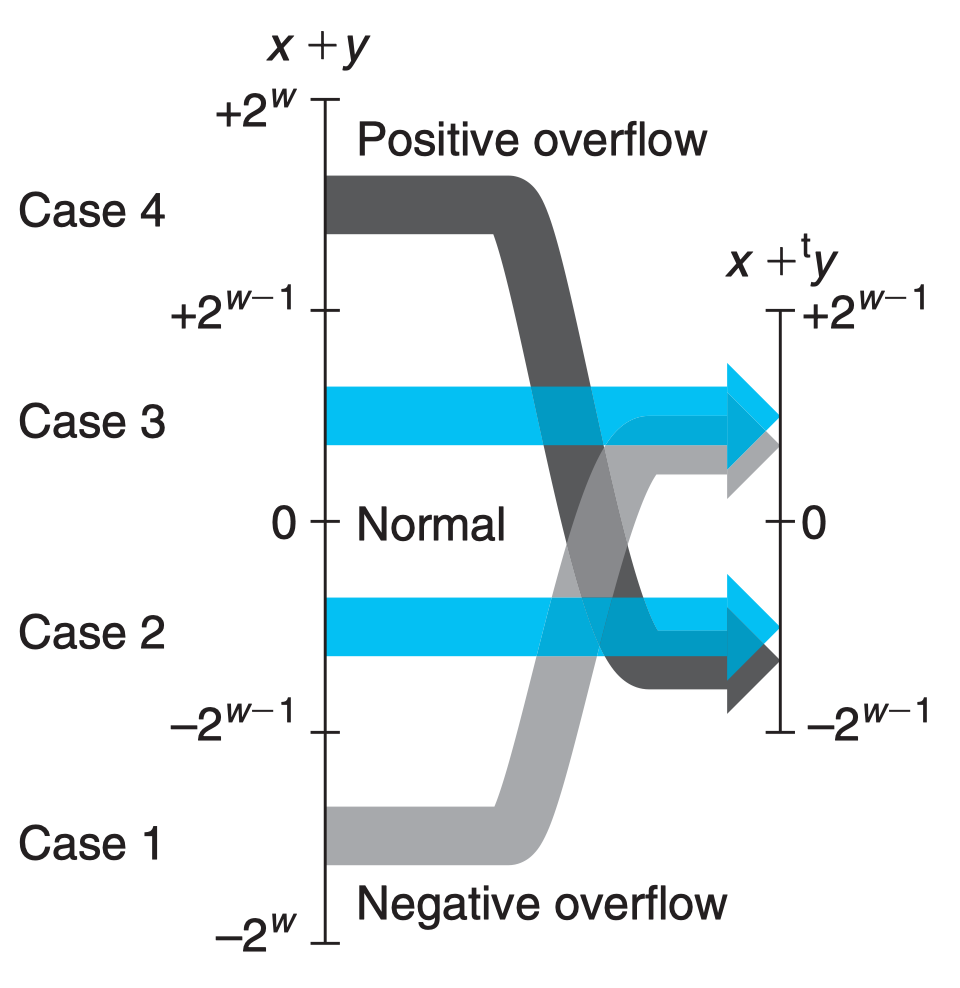
\includegraphics[width=0.3\linewidth]{ch2/figs/int_add_signed.png}
                                \caption{Results for unsigned (left) and signed (right) integer addition.}
                                \label{fig:intAdd}
                            \end{figure}
                    \end{outline}
                
                \subsection{Unsigned Multiplication}
                    \begin{outline}
                        \1 Unsigned integers in the range \( 0 \leq x, y \leq 2^w - 1 \) can be represented as \( w \)--bit numbers but their product could require \( 2w \) bits to represent
                        \1 Similar to addition, the result can be represented as product modulo \( 2^w \)
                            \[
                                x * \binom{u}{w}y = (x*y)~\text{mod}~2^w
                            \]
                    \end{outline}

                \subsubsection{Two's--Complement Multiplication}
                    \begin{outline}
                        \1 Most cases of two's--complement multiplication could fit into \( 2w -1 \) bits, but when the sum is \( 2^{2w - 2} \), it will require \( 2w \) bits
                        \1 Instead, we truncate the \( 2w \)-bit product to \( w \) bits
                            \[
                                x *\binom{t}{w}y = U2T_w \left( \left( xy  \right)~\text{mod}~2^w\right)
                            \]
                            \1 Given two w-bit vectors \( \hat{x} \) and \( \hat{y} \), the unsigned product \( B2U_w(\hat{x})*\binom{u}{w}B2U_w(\hat{y}) \) is identical in bit--level representation to the two's--complement product \( B2T_w(\hat{x})*\binom{t}{w}B2T_w(\hat{y}) \ \)
                            \2 Unsigned and two's--complement arithmetic is isomorphic, i.e. the operations \( +\binom{u}{w} \), \( -\binom{u}{w} \), and \( *\binom{u}{w} \) have the same bit--level effect as the operations \( +\binom{t}{w} \), \( -\binom{y}{w} \), and \( *\binom{t}{w} \)
                    \end{outline}

                    \subsubsection{Multiplication by Constants}
                        \begin{outline}
                            \1 \alert{important}: Integer multiplication is slow, requiring 10 or more clock cycles, as opposed to 1 clock cycle required by addition, subtraction, bit--level operations, and shifting.
                            \2 Compilers attempt to alleviate this by replacing multiplication by constants with combinations of shift and addition operations, called \gls{logShift}.
                            \1 The C/\Cpp~logical shift operation, \( x<<k \), is equivalent to \( x2^k \)
                            \1 As an example, in the expression \texttt{x * 14} 14 can be replaced with \( 14 = 2^3 + 2^w + 2^1 = \) \texttt{(x<<3) + (x<<2) + (x<<1)}, replacing one multiplication with three shift and two addition operations
                        \end{outline}

                    \subsubsection{Dividing by Powers of Two}
                        \begin{outline}
                            \1 Integer division is even slower than multiplication, requiring 30 or more clock cycles
                            \1 Division by a power of 2 can be performed using logical right shifts, \texttt{k>>x} is equivalent to \( x/2^k \)
                            \1 Division always rounds towards 0
                        \end{outline}
\end{document}
